\documentclass[11pt,a4paper]{article}
\usepackage[table]{xcolor}
\usepackage{geometry}
\geometry{a4paper, left=15mm, right=15mm, top=0mm, bottom=20mm}
\usepackage{graphicx}
\usepackage{tabularx}
\usepackage{titlesec}
\usepackage{tcolorbox}
\tcbuselibrary{skins}
\usepackage{helvet}
\renewcommand{\familydefault}{\sfdefault} % Sans serif font to match the web PDF

% Define Colors matching the HTML/CSS
\definecolor{techblue}{RGB}{30,58,138}
\definecolor{slatebg}{RGB}{240,244,248}
\definecolor{blueaccent}{RGB}{37,99,235}
\definecolor{darkslate}{RGB}{15,23,42}
\definecolor{cardborder}{RGB}{203,213,225}
\definecolor{highlightbg}{RGB}{239,246,255}
\definecolor{highlightborder}{RGB}{191,219,254}
\definecolor{tableodd}{RGB}{241,245,249}
\definecolor{tablehead}{RGB}{248,250,252}

% Set the full page background color
\pagecolor{slatebg}

% Format Sections (Adds the left blue accent border)
\titleformat{\section}
  {\normalfont\Large\bfseries\color{darkslate}}
  {}
  {0em}
  {\color{blueaccent}\vrule width 4pt\hspace{10pt}}
\titlespacing*{\section}{0pt}{0pt}{12pt}

% Setup custom tcolorbox for standard section cards
\newtcolorbox{sectioncard}{
    enhanced,
    colback=white,
    colframe=cardborder,
    boxrule=0.5pt,
    arc=4pt,
    drop shadow=black!5!white, % Subtle shadow
    left=20pt, right=20pt, top=15pt, bottom=15pt,
    boxsep=0pt,
    after skip=20pt
}

% Setup custom tcolorbox for the blue highlight box
\newtcolorbox{highlightbox}{
    enhanced,
    colback=highlightbg,
    colframe=highlightborder,
    boxrule=1pt,
    arc=4pt,
    left=15pt, right=15pt, top=10pt, bottom=10pt,
    boxsep=0pt,
    after skip=15pt
}

\setlength{\parindent}{0pt}
\setlength{\parskip}{8pt}

\begin{document}

% Full bleed tech-blue header
\begin{tcolorbox}[
    enhanced,
    colback=techblue,
    coltext=white,
    halign=center,
    valign=center,
    boxrule=0pt,
    arc=0pt,
    grow to left by=15mm,
    grow to right by=15mm,
    top=25mm,
    bottom=10mm,
    after skip=20pt
]
    {\huge\bfseries Research Summary \& Objectives\par}
    \vspace{6pt}
    {\large Design of an Authentication Mechanism for ECHONET Lite Based Smart Home Networks\par}
    \vspace{12pt}
    {\small Proposed by: Muhammad Suhaib | Supervisor: Prof. Dr. Selvakumar Manickam\par}
\end{tcolorbox}

\begin{sectioncard}
% \section*{1. Introduction \& Problem Statement}
% The Internet of Things (IoT) has become a primary driver of digital transformation, with Smart Home Environments (SHEs) standing out as one of the most rapidly expanding IoT deployments. Within these environments, communication protocols are heavily relied upon to facilitate interoperability between consumer electronics, sensors, and energy devices. Echonet Lite serves as a standardized, IP-based application-layer communication protocol specifically designed for smart homes and energy management systems.

% Despite its widespread adoption to enable cross-vendor interoperability, Echonet Lite inherently lacks a mandatory built-in authentication mechanism. Consequently, the protocol typically assumes a trusted local network environment or depends on optional external security measures. This absence of standardized freshness verification and authentication directly exposes constrained smart home devices to severe cyber threats, notably replay attacks, Denial of Service (DoS), and Economic Denial of Service (EDoS). Existing security alternatives are often neither lightweight enough nor fully standardized for such resource-constrained endpoints.

Over the past decade, the Internet of Things has quietly restructured the way people interact
with their homes. From air conditioners that respond to occupancy patterns to lighting managed
through a single application, Smart Home Environments (SHEs) have shifted from a niche idea
to something close to a standard expectation. As these deployments grow in scale, so does the
need for reliable, secure communication between the many devices that make them work.

Among the protocols developed to meet this demand, ECHONET Lite has carved out a meaningful
role in smart home and energy management systems. Operating at the application layer over IP
networks, it was built with cross-vendor interoperability as its primary design goal; a feature
that has made it especially relevant in markets where heterogeneous device ecosystems are the
norm rather than the exception.

Yet a closer look at the protocol reveals a structural concern that is easy to miss on first
inspection. ECHONET Lite does not enforce a mandatory authentication mechanism. It was
designed under the assumption that communication takes place within a trusted local network,
leaving any additional security to optional external layers. In practice, this means a receiving
device has no built-in way to confirm whether a message genuinely came from a legitimate
sender — or whether that same message has already been processed before.

This matters more than it might initially seem. Smart home devices are typically
resource-constrained, running on limited memory, processing power, and in many cases, battery
life. Simply layering on enterprise-grade security solutions is not a realistic option. And without
authentication or freshness verification at the protocol level, these devices are left exposed to a
set of attacks that are particularly problematic in IoT contexts. Replay attacks allow an adversary
to retransmit previously captured valid messages, triggering unintended device actions without
ever breaking encryption. Denial of Service (DoS) attacks flood devices with traffic until they
become unresponsive. Economic Denial of Service (EDoS) attacks take a different angle,
exploiting cloud-connected systems to drive up operational costs through sustained illegitimate
traffic. Existing alternatives whether DTLS or token-based schemes like JWT; are either too
computationally heavy for constrained endpoints or were never designed around the specific
structure of ECHONET Lite in the first place.

\end{sectioncard}

\begin{sectioncard}
\section*{2. Research Objectives}
To address the critical security vulnerabilities in the current Echonet Lite protocol, this research proposes the following primary objectives:
\begin{itemize}
    \item To propose a robust authentication mechanism for Echonet Lite that minimizes the reliance on optional external security layers, ensuring it remains highly suitable for constrained smart home devices.
    \item To formulate cryptographic protections specifically tailored for Echonet Lite capable of mitigating replay, DoS, and EDoS attacks while maintaining minimal performance overhead.
    \item To evaluate the proposed mechanism's processing time, control overhead, and attack prevention success rate against DoS, replay, and EDoS attacks.
\end{itemize}
\end{sectioncard}

\begin{sectioncard}
\section*{3. Methodology \& Experimental Scope}
The research is heavily design-oriented and experimental, structured into four strategic phases:
\begin{itemize}
    \item \textbf{Phase 1:} Identification of absent security features, focusing specifically on authentication and message freshness, alongside a structural analysis of the Echonet Lite protocol flow and object model.
    \item \textbf{Phase 2:} Development of a protocol-level authentication scheme, introducing a Security Extension Field (SEF) that maintains backward compatibility with the existing framework.
    \item \textbf{Phase 3:} Implementation of the proposed mechanism within a simulated Echonet Lite environment, modeling both the controller and end-device communication behaviors.
    \item \textbf{Phase 4:} Quantitative evaluation measuring the communication and processing overhead introduced by the new authentication fields, comparing the standard protocol against the newly authenticated variant.
\end{itemize}

The scope targets the Application Layer within a UDP/IP network environment. Evaluation metrics are strictly focused on processing time, control overhead, and the attack prevention success rate against DoS, replay, and EDoS attacks.

\begin{center}
    \fbox{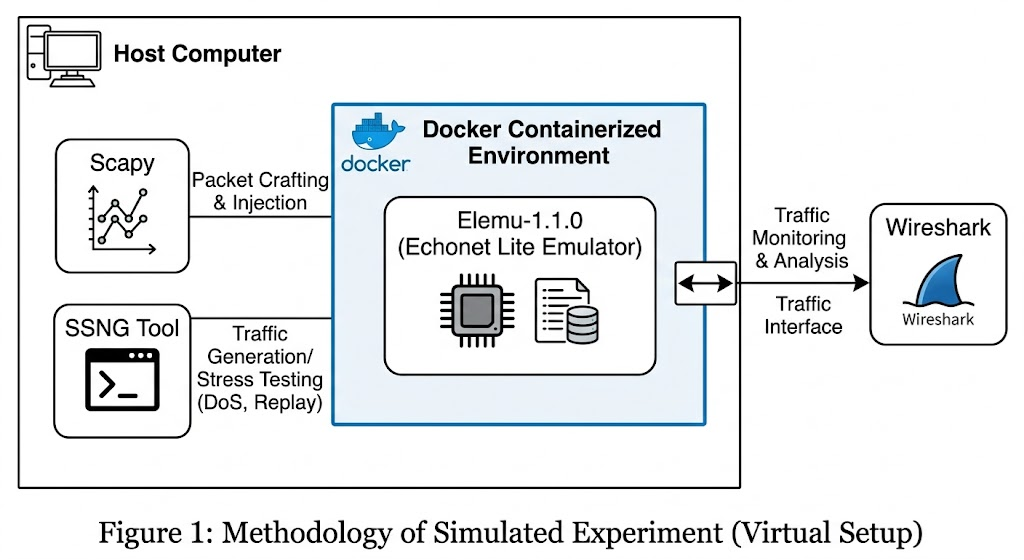
\includegraphics[width=0.85\textwidth]{assets/Experiment 1.png}} \\
    \vspace{4pt}
    \textit{\small Figure 1: Methodology of Simulated Experiment (Virtual Setup) utilizing Elemu-1.1.0, Docker, and Scapy for traffic generation and analysis.}
\end{center}
\end{sectioncard}

\begin{sectioncard}

  \begin{center}
    \fbox{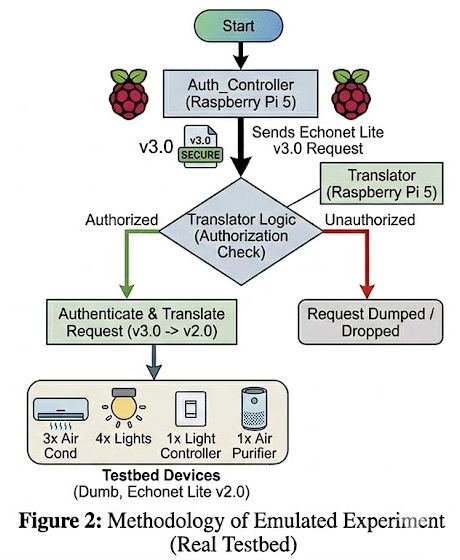
\includegraphics[width=0.85\textwidth]{assets/Experiment 2-Testbed Setup.png}} \\
    \vspace{4pt}
    \textit{\small Figure 2: Methodology of Emulated Experiment on a Real Testbed using Raspberry Pi controllers and physical smart home devices.}
\end{center}
\end{sectioncard}

\begin{sectioncard}

\section*{4. Preliminary Findings \& Expected Outcomes}
Initial implementation milestones successfully validated four distinct secure communication models for ECHONET-Lite environments. The quantitative analysis highlights the critical trade-offs between enhanced security and transmission overhead.

\vspace{10pt}
\rowcolors{2}{white}{tableodd}
\noindent
\begin{tabularx}{\textwidth}{|X|c|c|c|}
    \hline
    \rowcolor{tablehead}
    \textbf{Security Model} & \textbf{Avg. Total Size (B)} & \textbf{Avg. Payload (B)} & \textbf{Avg. Security Overhead (B)} \\
    \hline
    NATIVE (Baseline) & 20.40 & 20.40 & 0.00 \\
    \textbf{ELAF (Proposed)} & \textbf{44.72} & \textbf{21.72} & \textbf{23.00} \\
    DTLS (Standard) & 62.89 & 17.89 & 45.00 \\
    JWT (Token-based) & 148.40 & 20.40 & 128.00 \\
    \hline
\end{tabularx}
\vspace{15pt}

\begin{highlightbox}
    \textbf{Core Technical Contributions:}
    \begin{itemize}
        \item \textbf{Efficiency:} The proposed ECHONET Lite Authentication Framework (ELAF) is confirmed as the most efficient secure alternative. By introducing a Security Extension Field containing timestamps, counters, and HMACs, it adds merely 23 bytes of overhead per packet, drastically outperforming JWT (128B overhead).
        \item \textbf{Attack Resilience:} The integration of authentication on critical packet fields enables the immediate rejection of spoofed/malformed packets (mitigating DoS) and prevents unnecessary cryptographic processing, thereby protecting device battery and processing limits (mitigating EDoS). Monotonic counters and timestamps effectively detect and discard stale or maliciously replayed packets.
    \end{itemize}
\end{highlightbox}
\end{sectioncard}

\end{document}